% Este archivo es parte de la memoria del proyecto fin de carrera
% de Manuel López Urbina. Protegida bajo la licencia GFDL.
% Para más información, la licencia completa viene incluida en el
% fichero fdl-1.3.tex

% Copyright (C) 2012 Manuel López Urbina

\chapter{Guía de usuario}
\label{chap:manual-usuario}

\section{Introducción}

Este documento describirá los objetivos e información de cómo utilizar la aplicación junto con sus diferentes componentes hardware de: OpenTSR.\\

La aplicación OpenTSR ha sido creada por Manuel López Urbina para el proyecto fin de carrera de la titulación de ingeniería técnica informática de la universidad de Cádiz.\\

Resulta de vital importancia consultar esta guía antes y/o durante la utilización de los diferentes elementos tanto hardware como software del proyecto OpenTSR ya que le proporcionará una guía paso a paso en el manejo de sus funciones. La resolución recomendada para la aplicación debe ser superior o igual a 1024x768 (Estándar XGA).\\

Con el fin de facilitar la comprensión de la guía, se incorporan gráficos explicativos. Los diferentes iconos existentes en la aplicación han sido obtenidos de la página web \url{http://www.iconfinder.com}.

\subsection{Objetivo de esta guía}

Esta guía tiene como objetivo la de proporcionar al usuario un soporte de ayuda e iniciación a la utilización de los diferentes elementos hardware y software integrantes del proyecto OpenTSR. Esta sección comprende:

\begin{itemize}
\item Guía de acceso a la aplicación.
\item Guía de uso de la aplicación.
\item Guía para la puesta en marcha de los dispositivos hardware.
\item Guía para la configuración de los dispositivos hardware.
\end{itemize}

\subsection{Dirigido a}

Esta guía esta dirigida al usuario final del proyecto OpenTSR que utilicen como medio de control del vehículo \emph{Surveyor SRV-1 WiFi webcam robot} para proporcionarle de un sistema de visión artificial para el reconocimiento de señales de tráfico y de conducción autónoma.

\section{Obtener OpenTSR}

La aplicación se encuentra disponible en la forja \emph{rediris}\cite{website:iris} o usando la herramienta \emph{Subversion}\cite{librosvn}, escribiendo en la consola el siguiente comando:\\

\begin{lstlisting}[style=consola]
svn checkout https://forja.rediris.es/svn/opentsr
\end{lstlisting}

\section{Ingreso al sistema}

Una vez descargada la aplicación hacemos doble click sobre el icono para ejecutar la aplicación. Inmediatamente se mostrará la ventana principal mostrando el siguiente aspecto, ver Figura \ref{fig:ventana-principal}.\\

\begin{figure}[H]
  \begin{center}
    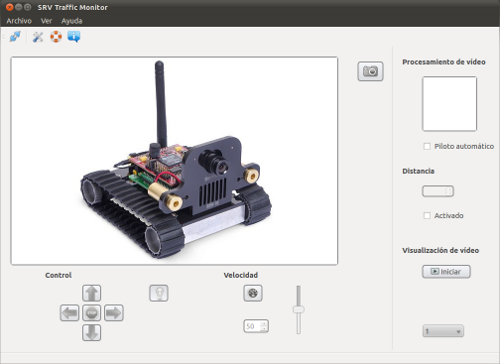
\includegraphics[scale=0.5]{ventana-principal.png}
  \end{center}
  \caption{Ventana principal de la aplicación.}
  \label{fig:ventana-principal}
\end{figure}

\section{Convenciones y estándares a utilizar}
\label{subsec:convenciones}

Las convenciones y estándares utilizados son los siguientes:

\subsubsection{Convenciones del uso del ratón}

\begin{table}[H]
\begin{tabular}{|p{2cm}|p{6cm}|p{6cm}|}
\hline
\centering{Término} & \centering{Elemento aplicación} & \qquad \quad Significado \\
\hline
\centering{ \vspace*{+.005in} 
\includegraphics[scale=0.7]{./imagenes/click_derecho.png}} & Sobre cualquier botón. & Apertura del menú o acción designado para tal botón. \\
\hline
\end{tabular}
\caption{Uso del ratón.}
\end{table}

\subsection{Convenciones del uso del teclado}
\label{sec:uso-teclado}

Para teclas simples:\\

\begin{table}[H]
  \begin{center}
    \begin{tabular}{|p{2cm}|p{10cm}|}
      \hline
      \centering{Tecla} & \qquad \quad Significado \\
      \hline
      
\includegraphics[width=2cm]{./imagenes/flecha_arriba.png} & \vspace*{-.8in}{Avanzar. Orden de movimiento frontal, el vehículo se detiene al soltar la tecla.} \\
      \hline
      
\includegraphics[width=2cm]{./imagenes/flecha_abajo.png} & \vspace*{-.8in}{Retroceder. Orden de movimiento en retroceso, el vehículo se detiene al soltar la tecla.} \\
      \hline
      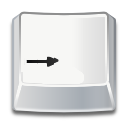
\includegraphics[width=2cm]{./imagenes/flecha_derecha.png} & \vspace*{-.8in}{Giro cerrado a la derecha. Orden de giro a la derecha, el vehículo se detiene al soltar la tecla.} \\
      \hline
      
\includegraphics[width=2cm]{./imagenes/flecha_izquierda.png} & \vspace*{-.8in}{Giro cerrado a la izquierda. Orden de giro a la izquierda, el vehículo se detiene al soltar la tecla.} \\
      \hline

      \hline
      
\includegraphics[width=2cm]{./imagenes/tecla_mas.png} & \vspace*{-.8in}{Incremento de velocidad. Se incrementa en una unidad la velocidad del vehículo.} \\
      \hline

      \hline
      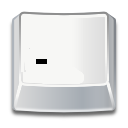
\includegraphics[width=2cm]{./imagenes/tecla_menos.png} & \vspace*{-.8in}{Disminución de velocidad. Se disminuye en una unidad la velocidad del vehículo.} \\
      \hline
    \end{tabular}
  \end{center}
\caption{Controles del teclado para teclas simples.}
\end{table}

\clearpage

Para combinaciones de teclas:\\

\begin{table}[H]
  \begin{center}
    \begin{tabular}{|p{6cm}|p{8cm}|}
      \hline
      \centering{Tecla} & \qquad \quad Significado \\
      \hline
      
\includegraphics[width=5.5cm]{./imagenes/flecha_arriba_y_derecha.png} & \vspace*{-.8in}{Giro abierto a la derecha. Orden de movimiento para la realización de un giro más abierto hacia la derecha. Los motores del vehículo mueven ambas cadenas aplicando a la derecha una menor velocidad. El vehículo se detiene al soltar ambas teclas o continua con el movimiento de la tecla que se sigue manteniendo pulsada.} \\
      \hline
      
\includegraphics[width=5.5cm]{./imagenes/flecha_arriba_e_izquierda.png} & \vspace*{-.8in}{Giro abierto a la izquierda. Orden de movimiento para la realización de un giro más abierto hacia la izquierda. Los motores del vehículo mueven ambas cadenas aplicando a la izquierda una menor velocidad. El vehículo se detiene al soltar ambas teclas o continua con el movimiento de la tecla que se sigue manteniendo pulsada.} \\
      \hline
      
\includegraphics[width=5.5cm]{./imagenes/flecha_abajo_y_derecha.png} & \vspace*{-.8in}{ Giro abierto a la derecha retrocediendo. Orden de movimiento para la realización de un giro más abierto hacia la izquierda marcha atrás. Los motores del vehículo mueven ambas cadenas aplicando a la izquierda una menor velocidad. El vehículo se detiene al soltar ambas teclas o continua con el movimiento de la tecla que se sigue manteniendo pulsada.} \\
      \hline
      
\includegraphics[width=5.5cm]{./imagenes/flecha_abajo_e_izquierda.png} & \vspace*{-.8in}{Giro abierto a la izquierda retrocediendo. Orden de movimiento para la realización de un giro más abierto hacia la izquierda marcha atrás. Los motores del vehículo mueven ambas cadenas aplicando a la izquierda una menor velocidad. El vehículo se detiene al soltar ambas teclas o continua con el movimiento de la tecla que se sigue manteniendo pulsada.} \\
      \hline
    \end{tabular}
  \end{center}
\caption{Controles del teclado para las combinaciones de teclas.}
\end{table}

\clearpage

\subsubsection{Convenciones del uso del gamepad}
\label{sec:convencion-gamepad}

\begin{table}[H]
  \begin{center}
    \begin{tabular}{|p{3cm}|p{8cm}|}
      \hline
      \centering{Botón} & \qquad \quad Significado \\
     \hline
      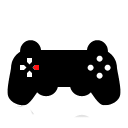
\includegraphics[width=3cm]{./imagenes/pad-2.png} & \vspace*{-.8in}{Giro cerrado a la derecha. Orden de giro a la derecha, el vehículo se detiene al soltar la cruceta.} \\
      \hline
      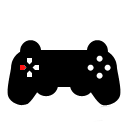
\includegraphics[width=3cm]{./imagenes/pad-4.png} & \vspace*{-.8in}{Giro cerrado a la izquierda. Orden de giro a la izquierda, el vehículo se detiene al soltar la cruceta.} \\
      \hline
       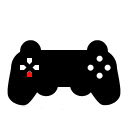
\includegraphics[width=3cm]{./imagenes/pad-3.png} & \vspace*{-.8in}{Retroceder. Orden de movimiento en retroceso, el vehículo se detiene al soltar la cruceta.} \\
      \hline
       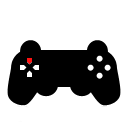
\includegraphics[width=3cm]{./imagenes/pad-1.png} & \vspace*{-.8in}{Avanzar. Orden de movimiento hacia delante, el vehículo se detiene al soltar la cruceta.} \\
      \hline
       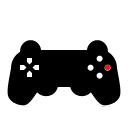
\includegraphics[width=3cm]{./imagenes/pad-6.png} & \vspace*{-.8in}{Sin función.} \\
      \hline
      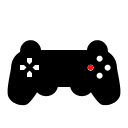
\includegraphics[width=3cm]{./imagenes/pad-8.png} & \vspace*{-.8in}{Disminuir velocidad. La velocidad de movimiento del vehículo disminuye.} \\
      \hline
    \end{tabular}
  \end{center}
\end{table}

\begin{table}[H]
  \begin{center}
    \begin{tabular}{|p{3cm}|p{8cm}|}
      \hline
       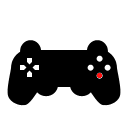
\includegraphics[width=3cm]{./imagenes/pad-7.png} & \vspace*{-.8in}{Incrementar velocidad. La velocidad de movimiento del vehículo aumenta.} \\
      \hline
       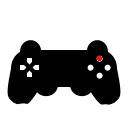
\includegraphics[width=3cm]{./imagenes/pad-5.png} & \vspace*{-.8in}{Sin función.} \\
      \hline
      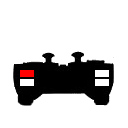
\includegraphics[width=3cm]{./imagenes/pad-9.png} & \vspace*{-.8in}{Tomar fotografía. Realiza una captura de la imagen visualizada en pantalla.} \\
      \hline
      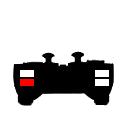
\includegraphics[width=3cm]{./imagenes/pad-10.png} & \vspace*{-.8in}{Sin función.} \\
      \hline
      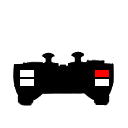
\includegraphics[width=3cm]{./imagenes/pad-11.png} & \vspace*{-.8in}{Activación/desactivación de láseres. Los láseres son desactivados si se encuentran en estado encendido o activados si se encuentran en estado apagado.} \\
      \hline
      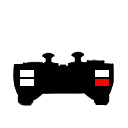
\includegraphics[width=3cm]{./imagenes/pad-12.png} & \vspace*{-.8in}{Sin función.} \\
      \hline
    \end{tabular}
  \end{center}
  \caption{Controles del gamepad.}
\end{table}


\section{Operaciones de la interfaz}
\label{sec:operaciones-interfaz}

En la ventana principal de la aplicación \ref{fig:ventana-principal}, se visualizan una serie de elementos, a continuación se describen cada uno de ellos.

\begin{itemize}
\item \textbf{Conectar:}\\
Icono representativo:\quad  \icontext{.4}{.5}{./imagenes/icono_conectar.png} \\
Acción: establece conexión con el vehículo SRV-1. Una vez accionado el botón cambia su estado pasando a \textbf{Desconectar}.

\item \textbf{Desconectar:}\\
Icono representativo:\quad  \icontext{.4}{.5}{./imagenes/icono_desconectar.png} \\
Acción: elimina la conexión con el vehículo SRV-1. Una vez accionado el botón cambia su estado pasando a \textbf{Conectar}.

\item \textbf{Activar láser:} \\
Icono representativo:\quad  \icontext{.4}{.3}{./imagenes/icono_laser_off.png} \\
Acción: activa los láseres del vehículo SRV-1. Una vez accionado el botón cambia su estado pasando a \textbf{Desactivar láser}.

\item \textbf{Desactivar láser:}\\
Icono representativo:\quad  \icontext{.4}{.3}{./imagenes/icono_laser_on.png} \\
Acción: desactiva los láseres del vehículo SRV-1. Una vez accionado el botón cambia su estado pasando a \textbf{Activar láser}.

\item \textbf{Tomar fotografía:}\\
 Icono representativo:\quad  \icontext{.4}{.15}{./imagenes/icono_foto.png} \\
Acción: toma una fotografía de la imagen visionada por la cámara.

\item \textbf{Velocidad alta:}\\
 Icono representativo:\quad  \icontext{.4}{.15}{./imagenes/icono_velocidad_alta.png} \\
Acción: asigna velocidad alta de desplazamiento al vehículo SRV-1. Una vez accionado el botón cambia su estado pasando a \textbf{Velocidad baja}.

\item \textbf{Velocidad baja:}\\
Icono representativo:\quad  \icontext{.4}{.15}{./imagenes/icono_velocidad_baja.png} \\
Acción: asigna velocidad baja de desplazamiento al vehículo SRV-1. Una vez accionado el botón cambia su estado pasando a \textbf{Velocidad alta}.


\item \textbf{Avanzar:}\\
Icono representativo:\quad  \icontext{.4}{.25}{./imagenes/icono_arriba.png} \\
Acción: ordena avanzar al vehículo, pulsar icono \emph{Stop} para detener o indicar nueva orden.

\item \textbf{Retroceder:}\\
Icono representativo:\quad  \icontext{.4}{.25}{./imagenes/icono_abajo.png} \\
Acción: ordena retroceder al vehículo, pulsar icono \emph{Stop} para detener o indicar nueva orden.

\item \textbf{Girar a la derecha:}\\
Icono representativo:\quad  \icontext{.4}{.25}{./imagenes/icono_derecha.png} \\
Acción: ordena realizar giro a la derecha al vehículo, pulsar icono \emph{Stop} para detener o indicar nueva orden.

\item \textbf{Girar a la izquierda:}\\
Icono representativo:\quad  \icontext{.4}{.25}{./imagenes/icono_izquierda.png} \\
Acción: ordena realizar giro a la izquierda al vehículo, pulsar icono \emph{Stop} para detener o indicar nueva orden.

\item \textbf{Parada:}\\
Icono representativo:\quad  \icontext{.4}{.3}{./imagenes/icono_stop.png} \\
Acción: ordena la parada del vehículo si se encontraba en movimiento.

\item \textbf{Información controles:}\\
Icono representativo:\quad \icontext{.4}{.5}{./imagenes/icono_controles.png} \\
Acción: abre una nueva ventana con información sobre los controles de la aplicación.

\item \textbf{Ayuda:}\\
Icono representativo:\quad \icontext{.4}{.5}{./imagenes/ayuda.png} \\
Acción: realiza la apertura de la guía de usuario de la aplicación.

Dentro de este documento se encuentran tres posibles opciones de consulta para el usuario.
\begin{itemize}
\item Guía de uso de la aplicación.
\item Guía hardware.
\item Sobre OpenTSR.
\end{itemize}

La guía de uso servirá para solventar las dudas de uso de la aplicación. En ella se hará un recorrido por todas las funcionalidades, así como los posibles usos que tiene cada componente de la misma.\\

En la guía hardware se describe paso a paso, la metodología a seguir para la configuración de los elementos hardware presentes en OpenTSR junto con pasos previos a su interconexión y puesta en funcionamiento de cada uno de ellos.

\item \textbf{Información:}\\
Icono representativo:\quad \icontext{.4}{.5}{./imagenes/informacion.png} \\
Acción: realiza la apertura de la ventana ``sobre OpenTSR'' que hace mención sobre el creador del proyecto, el nombre del mismo y para la universidad que ha sido desarrollada la aplicación.

\begin{figure}[H]
  \begin{center}
    
\includegraphics[scale=0.5]{sobreOpenTSR.png}
  \end{center}
  \caption{Ventana donde se visualiza la información relacionada con OpenTSR.}
  \label{fig:ventana-informacion}
\end{figure}


\item \textbf{Iniciar:}\\
Icono representativo:\quad \icontext{.4}{.5}{./imagenes/boton-iniciar.png} \\
Acción: Se inicia la conexión con la cámara mostrándose las imágenes en la interfaz. Una vez accionado se produce un cambio de estado del botón pasando a \textbf{Detener}.

\item \textbf{Detener:}\\
Icono representativo:\quad \icontext{.4}{.5}{./imagenes/boton-detener.png} \\
Acción: Se cierra la conexión con la cámara. Una vez accionado se produce un cambio de estado del botón pasando a \textbf{Iniciar}.

\item \textbf{Piloto automático}
checkbox \\
Acción: Se inicia el modo de pilotaje automático en el vehículo a partir de las señales de tráfico detectadas por el sistema, ver sección \ref{sec:operaciones-automatizadas} para consultar la relación entre señales detectables y acción automática realizada.

\end{itemize}

\section{Operaciones automatizadas}
\label{sec:operaciones-automatizadas}

Al activar el botón ``piloto automático'' en la interfaz gráfica se produce una conducción autónoma del vehículo a partir de las señales de tráfico visionadas por la cámara.\\

La correspondencia entre las señales detectables y su acción ejecutada se muestra en la siguiente tabla:\\

\clearpage

\begin{table}[H]
  \begin{center}
    \begin{tabular}{|p{2cm}|p{8cm}|}
      \hline
      \centering{Señal} & \qquad \quad Acción \\
      \hline 
\includegraphics[width=2cm]{./imagenes/1.jpg} & \vspace*{-.8in}{Orden automática de parada.} \\
      \hline 
\includegraphics[width=2cm]{./imagenes/2.jpg} & \vspace*{-.8in}{Velocidad fijada a 20*.} \\
      \hline 
\includegraphics[width=2cm]{./imagenes/3.jpg} & \vspace*{-.8in}{Velocidad fijada a 30*.} \\
      \hline 
\includegraphics[width=2cm]{./imagenes/4.jpg} & \vspace*{-.8in}{Velocidad fijada a 40*.} \\
      \hline 
\includegraphics[width=2cm]{./imagenes/5.jpg} & \vspace*{-.8in}{Velocidad fijada a 50*.} \\
      \hline 
\includegraphics[width=2cm]{./imagenes/6.jpg} & \vspace*{-.8in}{Velocidad fijada a 60*.} \\
      \hline 
\includegraphics[width=2cm]{./imagenes/7.jpg} & \vspace*{-.8in}{Velocidad fijada a 70*.} \\
      \hline 
\includegraphics[width=2cm]{./imagenes/8.jpg} & \vspace*{-.8in}{Velocidad fijada a 80*.} \\
      \hline 
\includegraphics[width=2cm]{./imagenes/9.jpg} & \vspace*{-.8in}{Velocidad fijada a 90*.} \\
      \hline
   \end{tabular}
  \end{center}
\end{table}

\begin{table}[H]
  \begin{center}
    \begin{tabular}{|p{2cm}|p{8cm}|}
      \hline 
\includegraphics[width=2cm]{./imagenes/10.jpg} & \vspace*{-.8in}{Velocidad fijada a 100*.} \\
      \hline 
\includegraphics[width=2cm]{./imagenes/11.jpg} & \vspace*{-.8in}{Efectúa un giro cerrado a la derecha.} \\
      \hline 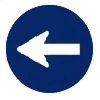
\includegraphics[width=2cm]{./imagenes/12.jpg} & \vspace*{-.8in}{Efectúa un giro cerrado a la izquierda.} \\
      \hline
    \end{tabular}
  \end{center}
  \caption{Señales reconocidas por el vehículo junto con la acción realizada.}
\end{table}

\begin{fondo}
  \begin{nota}
    Las velocidades son asignadas al vehículo dentro de una escala de 0 a 100, siendo 0 la velocidad nula y 100 su velocidad máxima.
  \end{nota}
\end{fondo}

\section{Montaje del sistema de comunicaciones}
\label{sec:montaje-sistema-comunicaciones}

En esta sección se detallada el montaje del sistema de comunicaciones entre el coche y el ordenador personal para su utilización.\\

Primeramente se realiza la conexión del router inalámbrico enchufando el adaptador de corriente a una toma de 220V y presionando el botón de encendido. Tras la espera de unos segundos escanearemos con un ordenador las conexiones WiFi existentes para proceder a conectarnos a la red de nuestro router, en este caso SRV-1. Si el router no ha sido configurado previamente visite la sección \ref{sec:configuración-router}.\\

El siguiente paso consiste en conectar el sistema de recepción de imágenes al ordenador personal. Para ello, se enchufa el adaptador de corriente del dispositivo sintonizador a la toma de 220V y éste, a su vez con la capturadora de vídeo mediante los cables RCA. Finalmente se conecta el cable USB de la capturadora de vídeo al ordenador personal tal y como muestra la figura \ref{fig:todo-conectado}. Si no se han instalado los drivers de la capturadora de vídeo visite la sección \ref{sec:drivers-capturadora}.\\

\begin{figure}[H]
  \begin{center}
    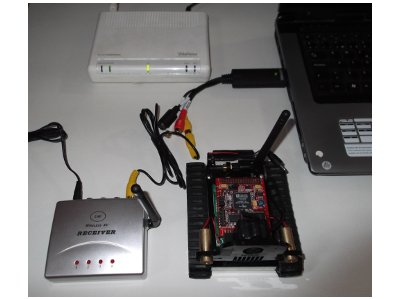
\includegraphics[scale=0.8]{elementos-hardware.jpg}
  \end{center}
  \caption{Vista de los elementos conectados.}
  \label{fig:todo-conectado}
\end{figure}


Una vez realizadas las conexiones, en el siguiente paso se debe sintonizar el sistema de recepción de imágenes para la captura de las imágenes de la cámara inalámbrica. Para ello desplazamos el interruptor hacia cada una de sus posiciones hasta obtener una imagen nítida y legible como la que se aprecia en la figura \ref{fig:im-ok}.\\

\begin{figure}[H]
  \begin{center}
    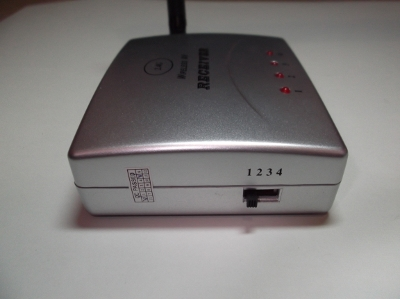
\includegraphics[scale=0.5]{interruptor.jpg}
  \end{center}
  \caption{Interruptor para búsqueda del canal de la cámara.}
  \label{fig:im-ok}
\end{figure}

\begin{figure}[H]
  \begin{center}
    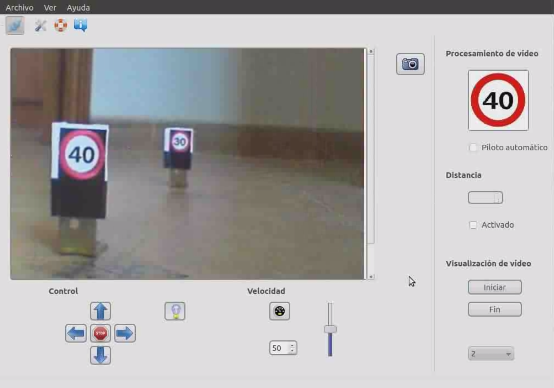
\includegraphics[scale=0.5]{todo-ok.png}
  \end{center}
  \caption{Vista de OpenTSR en funcionamiento.}
  \label{fig:im-ok}
\end{figure}

Por último, se debe realizar el encendido del vehículo robótico SRV-1 Surveyor accionando el interruptor situado en la parte trasera del mismo. Ver figura \ref{fig:interruptor-srv}. Si el robot no ha sido configurado para localizar el router y formar parte de la infraestructura de red visite la sección \ref{sec:configuración-srv}.\\

\begin{figure}[H]
  \begin{center}
    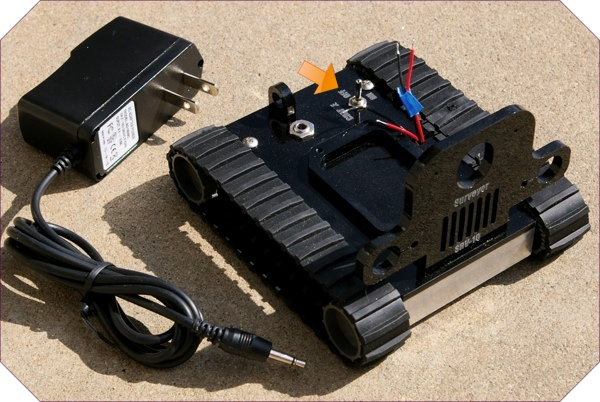
\includegraphics[scale=0.5]{quad-base-interruptor.jpg}
  \end{center}
  \caption{Localización del interruptor con tres modos de funcionamiento del robot SRV-1.}
  \label{fig:interruptor-srv}
\end{figure}

Finalmente pulse sobre el botón conectar de la aplicación (\icontext{.4}{.5}{./imagenes/icono_conectar.png}) para establecer conexión con el vehículo y proceder a su utilización.\\

A partir de este momento el sistema hardware se encuentra conectado y listo para ser usado por sistema software, del que se detalla los controles y su funcionamiento en el punto \ref{sec:operaciones-interfaz} y \ref{subsec:convenciones}.

\section{Configuración del router}
\label{sec:configuración-router}

El router actúa de intermediario entre el ordenador y el vehículo robótico, por tanto, dicho router debe ser configurado de tal manera de que que disponga de la misma dirección ip que ha sido introducida como puerta de enlace en la configuración del SRV-1 entre otros factores.\\

Para proceder con la configuración del router, primeramente, debemos conectar un extremo de un cable Ethernet a nuestro equipo y el otro a una de las interfaces Ethernet que dispone el router en su parte trasera.\\

Una vez conectado, para acceder al programa de configuración, basta con teclear en la barra de direcciones de nuestro navegador la dirección IP del router, debemos tener en cuenta que la dirección será 192.168.1.1 si el router posee su configuración por defecto, si hemos modificado la dirección ip, habrá que teclear la que corresponda.\\

Para consultar la dirección ip del router introducimos en terminal el siguiente comando:\\

\begin{lstlisting}[style=consola]
ifconfig
\end{lstlisting} 

Localizamos nuestra tarjeta y visualizamos la ip correspondiente a la puerta de enlace, la cual se corresponderá con la dirección de nuesto router.\\

La configuración por defecto del router tiene los siguientes valores: 

\begin{itemize}
\item Usuario: 1234 
\item Password: 1234 
\item Dirección IP: 192.168.1.1 
\item Red inalámbrica: deshabilitada 
\item Servidor DHCP: habilitado, dirección IP inicial 192.168.1.33 , dirección IP final 192.168.1.254 
\end{itemize}

Una vez hemos accedido al menú de configuración del router debemos configurar los siguientes parámetros:

\begin{itemize}
\item Habilitar la red inalámbrica.
\item Asignar como SSID del router SRV-1.
\item Establecer como dirección ip del router la 75.15.156.1.
\item Establecer como máscara de subred la ip 255.255.255.0.
\item Habilitación de contraseña de red inalámbrica según preferencia.
\end{itemize}

\begin{fondo}
  \begin{nota}
    es importante recordar los parámetros configurados en el router para establecer la configuración del vehículo SRV-1 compatible con la del router. 
  \end{nota}
\end{fondo}

\section{Configuración del vehículo SRV-1}
\label{sec:configuración-srv}

\subsection{Configuración del MatchPort}

El vehículo SRV-1 debe ser configurado para que, tras su encendido, localice automáticamente el router y establezca conexión con el mismo formando parte de una infraestructura de red.\\

Para acceder al menú de configuración MatchPort es necesario disponer de una interfaz serial de 3,3V como la mostrada en la imagen \ref{fig:placa-configuracion}\\

\begin{figure}[H]
  \begin{center}
    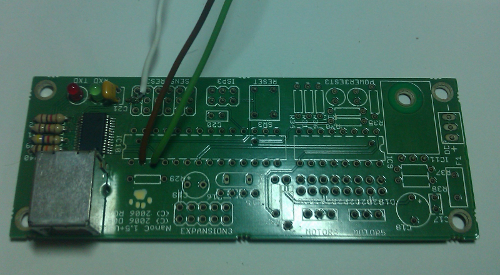
\includegraphics[scale=0.5]{placa-configuracion.png}
  \end{center}
  \caption{Imagen de la placa de configuración.}
  \label{fig:placa-configuracion}
\end{figure}

Se procede a la retirada la tarjeta Blackfin situada en la parte superior del SRV-1 para realizar la conexión con el puerto de expansión de 32 pines tal y como se muestra en la imagen \ref{fig:conexion-placa}.\\

\begin{figure}[H]
  \begin{center}
    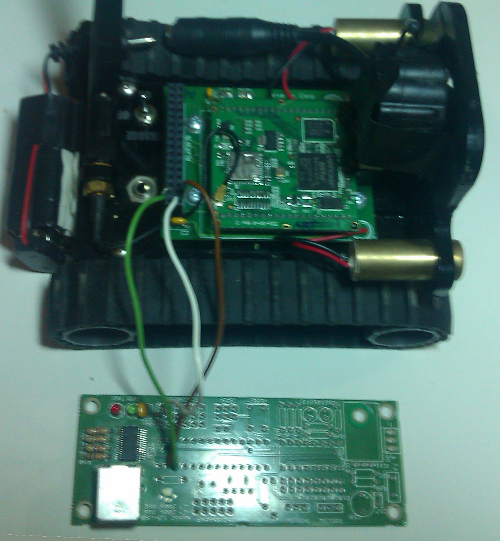
\includegraphics[scale=0.4]{conexion-placa.png}
  \end{center}
  \caption{Conexión de la placa al SRV-1.}
  \label{fig:conexion-placa}
\end{figure}

A continuación conecte la placa mediante el uso de un cable USB al ordenador. Los controladores del controlador CP2102 están integrados en Linux así que no es necesario instalar drivers adicionales. \\

Para configurar el MatchPort, inicie un programa terminal para que establezca conexión con la placa USB, para ello debemos ajustar la velocidad en 9600 baudios, encienda el robot y rápidamente (en unos pocos segundos) teclee 3 veces el carácter 'x', tras este paso se obtendrá en pantalla el menú de configuración para la MatchPort. Ver figura \ref{menu-matchport}.\\

\begin{figure}[H]
  \begin{center}
    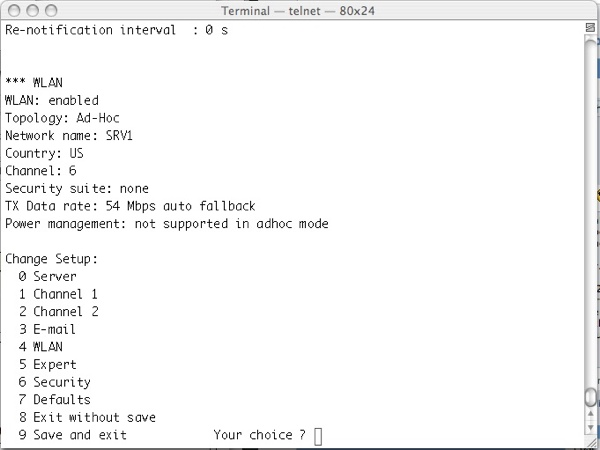
\includegraphics[scale=0.4]{matchport-config3.jpg}
  \end{center}
  \caption{Menú de configuración del Matchport.}
  \label{menu-matchport}
\end{figure}

Al restaurar el MatchPort a 2500kbps, los cambios a realizar son:

\begin{enumerate}
\item Experto (5)
  \begin{itemize}
  \item Rendimiento de la CPU, se introduce el valor FF
  \item Valores de  clk, se introduce el valor 81.
  \item Tamaño de MTU, pasamos de 1400 a 1024.
  \item Se omiten el resto de opciones.
  \end{itemize}
\item WLAN (4) 
  \begin{itemize}
  \item Establecemos un ssid, SRV-1
  \item Seleccionamos red de infraestructura.
  \item Canal 1 de serie (1).
  \item Baudrate, escriba -1.
  \item Divisor, introduzca 2.
  \item Control de flujo, introduzca 2.
  \item FlushMode, introduzca 80.
  \item para el paquete de Cntrl, introduzca C0
  \item Hora InterCh, introduzca 3
  \item Se omiten el resto de opciones.
  \end{itemize}
\item Network (0) 
  \begin{itemize}
  \item Se establece la dirección IP, Se asigna la 75.15.156.238, máscara: 255.255.255.0.
  \end{itemize}
\item Guardar y salir (9)
\end{enumerate}

\begin{fondo}
  \begin{nota}
    Para usuarios Windows el programa Hyperterminal presenta problemas. Se recomienda utilizar en Windows el programa Br@y Terminal.
    Para usuarios Linux se recomienda la utilización de PuTTY.
  \end{nota}
\end{fondo}

\begin{fondo}
  \begin{nota}
    El módulo WLAN MatchPort es un dispositivo de 3.3V. Si tratas el MatchPort con una interfaz serial RS232 (+ /-12V niveles), es probable que dañe la placa MatchPort y quede inutilizada.
  \end{nota}
\end{fondo}

\subsection{Carga de batería del vehículo SRV-1}

Para la carga de batería se debe conectar el adaptador jack al vehículo y el enchufe a una toma de 220V, es necesario utilizar un conversor del sistema Americano al Europeo. Ver figura \ref{fig:adaptador-corriente}.\\

\begin{figure}[H]
  \begin{center}
    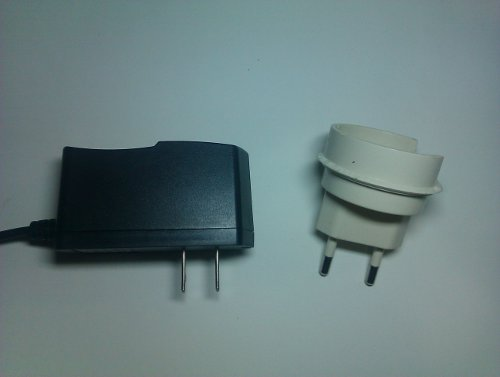
\includegraphics[scale=0.5]{adaptador-corriente.jpg}
  \end{center}
  \caption{Adaptador de corriente para realizar cargas de batería en el robot SRV-1.}
  \label{fig:adaptador-corriente}
\end{figure}

Posteriormente encender el vehículo SRV-1 en modo carga, \emph{charge}, mostrando el adaptador de corriente el led en color rojo. EL periodo de carga es de una hora de duración. Ver figura \ref{fig:interruptor-srv}.\\

\section{Instalación de la capturadora}
\label{sec:drivers-capturadora}

La capturadora de vídeo es el dispositivo conversor de la imagen de analógico a digital, para, posteriormente ser captada por el ordenador. En esta guía se detalla el proceso de instalación de los drivers en una distribución Ubuntu.\\

Los drivers son incluidos en la versión Ubuntu 12.04 LTS siendo innecesario realizar los pasos indicados en esta guía. Si dispones de una versión de Ubuntu anterior, proceda a la realización de los pasos aquí indicados:

\begin{enumerate}
\item Primeramente conecte el dispositivo a un puerto USB de su equipo e introduzca en una terminal el siguiente comando:
  \begin{lstlisting}[style=consola]
    lsusb
  \end{lstlisting}
  
  Entre los dispositivos detectados debe existir la siguiente línea:
  
  \begin{lstlisting}[style=consola]
    USB ID 05e1:0408
    Bus 002 Device 017: ID 05e1:0408 Syntek Semiconductor Co., Ltd
  \end{lstlisting}
  
\item Una vez comprobado que el dispositivo se corresponde con el del driver desconéctelo de su puerto USB. Para comenzar con la instalación se debe previamente descargar el driver, para ello introduzca en una terminal:
  
  \begin{lstlisting}[style=consola]
    wget http://sourceforge.net/projects/easycapdc60/files/easycap\_dc60.0.9.tar.gz/download => \ `easycap\_dc60.0.9.tar.gz`
  \end{lstlisting}
  
\item Instalamos los paquetes necesarios:
  \begin{lstlisting}[style=consola]
    \$ sudo apt-get install linux-headers-\$(uname -r) build-essential
  \end{lstslisting}
  
\item Para descomprimir el driver:
  \begin{lstlisting}[style=consola]
    mkdir ~/EASYCAP
    cd ~/EASYCAP
    cp -p ~/Desktop/easycap\_dc60.x.y.tar.gz .
    tar zxvf easycap\_dc60.0.9.tar.gz  
    cd easycap\_dc60.0.9.tar.gz
  \end{lstlisting}
  
\item En el directorio donde se extrajo el archivo .tar, introduzca el siguiente comando para instalar el driver:
  
  \begin{lstlisting}[style=consola]
    sudo ./install.sh
  \end{lstlisting}
  
\item Después de que la instalación haya finalizado, compruebe que el módulo ha sido cargado satisfactoriamente en el kernel mediante el uso del siguiente comando:
  
  \begin{lstlisting}[style=consola]
    lsmod | grep easycap
  \end{lstlisting} 
  
\item Ahora conecte en el puerto USB el dispositivo y compruebe que ha sido detectado, mediante el uso del siguiente comando:
  \begin{lstlisting}[style=consola]
ls /dev/easy*
  \end{lstlisting}
  
  Si todo funcionó correctamente, se debería visualizar algo como lo siguiente:
  \begin{lstlisting}[style=consola]
    /dev/easycap0
    /dev/easysnd1/
  \end{lstlisting}
  
\end{enumerate}

